\documentclass{article}
\usepackage[utf8]{inputenc}
\usepackage[margin=0.8in]{geometry} 
\usepackage{algorithm}
\usepackage{amsmath}
\usepackage{indentfirst}
\usepackage{amsmath}
\usepackage{graphicx}
\usepackage{subcaption}
\usepackage[table,xcdraw]{xcolor}
\usepackage[noend]{algpseudocode}

\graphicspath{ {./images/} }

\title{\textbf{Tour Mate App}}
\author{
    Alexandre Abreu\\
    \texttt{up201800168@fe.up.pt}
    \and
    Eduardo Correia\\
    \texttt{up201806433@fe.up.pt}
    \and
    Juliane Marubayashi\\
    \texttt{up201800175@fe.up.pt}
}

\renewcommand{\today}{\ifcase \month \or January\or February\or March\or %
April\or May \or June\or July\or August\or September\or October\or November\or %
December\fi, \number \year}
\date{
    Faculdade de Engenharia da Universidade do Porto\\
    \today
}

\begin{document}

\maketitle

\section*{Keywords}

Tourism, Graph Theory, Network Graph

\section*{Abstraction} 
    The goal of this project is to build the \textit{TourMateApp} application. \par 
    This hypothetical application's purpose is to generate adaptable urban tourist routes, according to the personal preferences of its user.\par
    The methodology must use an implementation of graphs to get the values.

\section*{Introduction}
\subsection*{Problem Description}
    The problem discussed in this paper is how to evaluate the best tourist path to a client that is in a specific place and has limited time to spend, taking into account his preferences.\par
    We must take into account the time spent in commutations and the expected time of visits. \par
    For example reasons, we used the Porto city as a reference model to work on.

\section*{Model Formulation}
\subsection*{Edge Weight}
    The maximum speed and the distance to travel along an edge are used to calculate the cost of moving between two nodes, assuming there will be no interaction with other vehicles or people. \par
    
\subsection*{Input Data}
G = (V, E) - dense weighted directed graph:
\begin{itemize}
\item V - set of nodes representing points in the map:
    \begin{itemize}
    \item ID - unique, the id of the node in the Open Street Map.
    \end{itemize}

\item $E_i$ - edge representing a path between two nodes that is identified by the OSMid = i:
    \begin{itemize}
    \item $OSM id$ - the id of the edge in the Open Street Map. 
    \item $S_i$ - The id of the source node.
    \item $T_i$ - The id of the target node.
    \item $L_i$ - Length of the road.
    \item $M_i$ - The maximum speed of the road.
    \item $O_i$ - True if the street is just one way, False otherwise.
    \end{itemize}
\end{itemize}

Input POI
\begin{itemize}
    \item $ID$: Id of the Vertex 
    \item $Name$: Name of the POI 
    \item $Time$: Avarage time that a person spends in that place
\end{itemize}

\subsection*{Input extraction from csv}
To initially obtain the map data from OSMnx \cite{OSMnx} we used a Python library that retrieves, models, analyzes, and visualizes street networks and other spatial data from OpenStreetMaps \cite{OpenStreetMaps}. \par
On that way, we can easily obtain a visual representation of streets and locations much like a graph - in which the crossings/POIs would be vertexes and the streets would be edges - and export it to a file our algorithm could parse. \par
Furthermore, the user would inform about its preferences, according to its trip purpose (recreational, work...), such as the list of POIs to visit, the maximum total time available to spend, the type of circuit (by foot, bicycle, car, public transportation...).

The input data includes \textit{.csv} files (obtained with OMSnx library \cite{OSMnx} and cleaned with Pandas \cite{Pandas}) stores information about the edges and nodes. \newline

\subsection*{Output Data}
    \subsubsection*{Output data available for the user}
    \begin{itemize}
        \item The path to pass by in order to achieve the points of interest as the path line shown on the map.
        \item Name of the streets and directions needed to be followed in respective order.
        \item The total time to be spent by the tourist, including visiting the POIs, and in the way to get to the places.
        \item The total distance to go. 
    \end{itemize}
    
    \subsubsection*{Output data after loading files}
    After reading the \textit{.csv} file with edges and nodes information, a \textit{Dense Direct Graph} $G(V,E)$ will be built with $V$ vertexes and $E$ edges.
    

\begin{itemize} 

    \item $E_i$
    \begin{itemize}
        \item $S_{ref}$: source node reference 
        \item $T_{ref}$: target node reference
        \item $w_{ij}$: calculated by $max\_velocity/road_{lenght}$
        \item name: name of the street
    \end{itemize}
    
    \item V
    \begin{itemize}
        \item $id$: vertex number identification.
        \item $Adj_i: $ adjacent list for a vertex i.
        \item $t$: average time spent in the POI.
    \end{itemize} 
 
\end{itemize}       

\subsubsection*{Output after loading data about POIs}
    A class containing all the POI's will be built 
\begin{itemize}

    \item POI
    \begin{itemize}
        \item $ID$: Id of the Vertex 
        \item $Name$: Name of the POI 
        \item $Time$: Avarage time that a person spends in that place
    \end{itemize}
    \item $POIs$: Hashtable(string, POI) containing all the POIs.
    \item $CityName$: Name of the city with the POI's stored.
    \end{itemize}
    

\subsection*{Objective Function}

The optimal solution of the problem resides in minimizing the total time spent in commuting and the total traveled time and maximizing the number of points of interest visited. \newline
\begin{itemize}
    \item $T_{total}$ is the amount of time the user has to spend
    \item $d_{ij}$ is the distance between point i and point j
    \item $v_{ij}$ if the allowed between point i and j 
    \item $POI$ is the set of points of interest visited (POI)
    \item $t_i$ is the time spent in a POI
\end{itemize}

$$f = min(\sum_{i,j \in POI}{\frac{d_{ij}}{v_{ij}}}) \times min(\sum_{i \in POI}{t_i}) \wedge min(\sum_{i \in POI}{t_i}) <= T_{total}$$
\and

\subsection*{Constraints}
\begin{itemize}
    \item $\lambda(i,j) > 0 \text{, } \forall (i,j) \in E$   
    \item $ g > 0 \wedge f > 0$
    \item $T_{i} \neq NIL \wedge T_{ref} > 0 \text{, } \forall T_{ref} \in V$
    \item $S_{i} \neq NIL \wedge S_{ref} > 0 \text{, } \forall S_{ref} \in V$
    \item $L_{i} > 0$
    \item $M_i > 0$
\end{itemize}

\section*{Identification of Supported Cases}
    Considering the initial options given in the main menu of the application, the supported cases includes: 
    \begin{itemize}
        \item Just one type of locomotion: car. However the algortihm could work for any time of locomotion. 
        \item The client can choose the points of interesting 
        
    
    \end{itemize}
\section*{Conectivity of the maps implemented} 
    \begin{itemize}
        \item All the graphs implemented were heavy graph, since all the edges have weight.
        \item The maps used for the project are all connected, since from one node we can reach all the others. 
    \end{itemize}
    
\section*{Solution Description}

\subsection*{Pre-processing}
    The main algorithm to be used in the application is the \textit{Floyd Warshall} \cite{IntroductionToAlgorithms} \cite{FloydWarshal}. \par
    
    \begin{algorithm}[h]
    \caption{Floyd-Warshall}
    \begin{algorithmic}[1]
    \Procedure{Shorthest Path}{G=(V, E)}
        \State $dist \gets N \times N \text{ matrix}$

        \For{\textbf{each} $\text{vertex } v \in dist$}
            \State $dist[i][i] \gets 0$
        \EndFor
        
        \For{\textbf{each} $\text{edge } w \in dist$}
            \State $dist[u][v] \gets weight(u, v)$
            \State $pred[u][v] \gets origin(w)$ 
        \EndFor
        
        \For{k \textbf{from} 1 \text{to} V}
            \For{i \textbf{from} 1 \text{to} V}
                \For{j \textbf{from} 1 \text{to} V}
                    \If{dist[i][j] $>$ dist[i][k] + dist[k][j]} 
                        \State dist[i][j] = dist[i][k] + dist[k][j]
                        \State pred[i][j] = pred[k][j];
                    \EndIf
                \EndFor
            \EndFor
        \EndFor
    \EndProcedure
    \end{algorithmic}
\end{algorithm}

    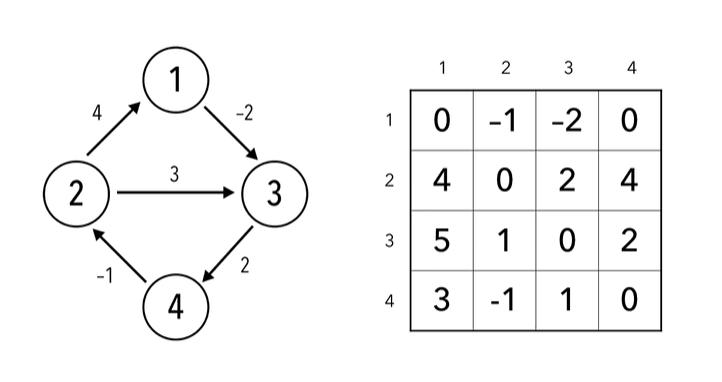
\includegraphics{algorithm-diagram}

    This algorithm considers the intermediate nodes to find and store all the shortest \b{distance} between nodes $i$ and $j$ with $k$ as intermediate vertex ($i \rightarrow k \rightarrow j$, which can simply described by the recursion formula: 
    
    \begin{equation} 
      d_{ij}^{(k)} =
        \begin{cases}
          w_{ij} & \text{if k = 0}\\
          min(d_{ij}^{k-1}, d_{ik}^{k-1} + d_{ki}^{k-1}) & \text{if } k\>= 1\\
        \end{cases}       
    \end{equation}
    
    Besides the $O(|V^3|)$ complexity, this is a good approach for dense graphs like city networks.
    However, the \textit{Floyd Warshall} algorithm doesn't store the path between nodes. To do so, we can consider a new matrix called $\Pi$ $(pred)$. \par
    For each $d_{ij}^{k}$ element in the matrix of shortest path $D^k$ the matrix $\Pi$ $(pred)$ will contain the respective shortest path for the pair of nodes $i$ and $j$. \par
    Formally, each element of $\Pi$ can be described as it follows for $k>1$:
    
    \begin{equation} 
      \pi_{ij}^{(k)} =
        \begin{cases}
          \pi_{ij}^{k-1} & \text{if } d_{ij}^{k-1} <= d_{ik}^{k-1} + d_{kj}^{k-1} \\
          \pi_{kj}^{k-1} & \text{if } d_{ij}^{k-1} > d_{ik}^{k-1} + d_{kj}^{k-1}\\
        \end{cases}       
    \end{equation}
    
    For $k = 0$ the definition will be: 
    
    \begin{equation} 
      \pi_{ij}^{(0)} =
        \begin{cases}
          NIL & \text{if } w = \inf \vee \text{ i = j}\\
          i & \text{if } i \neq j \wedge w < \inf\\
        \end{cases}      
    \end{equation}
    
    To complete the algorithm analysis, the spacial complexity for this algorithm should be $O(|v^2|)$, since it uses two auxiliary N $\times$ N matrices. \newline 
    In order to make the waiting time less significant, improvements to this algorithm will be considered. 

\subsection*{Choose the next vertex}
After calculating all the minimum distance between all the pairs of vertices, it's necessary to define a strategy to choose the next vertex. 

\subsubsection*{Greedy approach}
\begin{itemize}
    \item \textbf{vPOI} is the \textbf{vector of pointers} containing the points of interest represented by the POI structure defined previously.
    \item \textbf{maxTime} is a variable containing the maximum time that a person can spend.
    \item \textbf{origin} parameter represents the position of the initial point at vPOI. 
    \item Always consider the \textbf{vPOI[0]} as the initial point.
\end{itemize}

Remember that the index of a $origin$ vertex in vPOI is not the same index of this same vertex in the vector of vertices in the graph. 


    \begin{algorithm}[h]
    \caption{Greedy approach - Pre Processing}
    \begin{algorithmic}[1]
    \Procedure{trajectoryOrder}{vPOI, maxTime, G=(V,E)}
        \State $order \leftarrow \text{ vector}$ \Comment{Will store the final sequence of vertex}
		\State $visited \leftarrow |V| \text{ vector}$
        \State $idNext \leftarrow int$ \Comment{Id of next POI to be visited} 
        \State $initalTime \gets maxTime - \text{time spend in the origin POI}$
        \State $ $
        \State $indexOrigin \gets \text{finds index of origin in V}$
        \State $visited[indexOrigin] = true$  
        
        \State $ $
        
        \For{\textbf{each} $\text{poi } p \in vPOI$}
            \State $idNext \gets nextPoi\text{(indexOrigin, vPOI, visited, initialTime)}$ 
            \State $ $
            \If {$idNext = -1$}
            \Return $order$ \Comment{Don't have time to visit any other POI} 
            \EndIf
            \State $ $
            \State $originPos \gets \text{finds origin index in V}$
            \State $nextPos \gets \text{find idNext index in V}$
            \State $FloydPath \gets getFloydPath(\text{originPos, nextPos})$
            \State $ $
            \State $order \gets order[0... |order|-1] + FloydPath[0...|FloydPath|-1]$ \Comment{Add path to the next POI}
            \State $ $
            \State $visited[idNext] = true$  
            \State $origin \gets idNext$
        \EndFor
    \State $ $
    \Return order
    \EndProcedure
    \end{algorithmic}
\end{algorithm}
\newpage

    \begin{algorithm}[h]
    \caption{Main Greedy Approach}


    \begin{algorithmic}[1]
    \Procedure{NextPoi}{originIndexV, vPOI, visited, maxTime, G=(V,E)}
        \State $actualVertexIndex \gets originIndexV $
        \State $minWeight \gets \infty$
        \State $ $
        \State $selectedIndexVPOI \gets -1$
  
        
        \State $ $
        
        \For{i \textbf{from} 0 \text{to} $|$vPOI$|-1$}
            \State $nextVertexIndex \gets \text{finds vPOI[i] index in V}$ 
            \State $time \gets \text{finds the time to be spent in vPOI[i]}$
            
            \State $ $
            \If{dist[actualVertexIndex][nextVertexIndex] + time $<$ minWeight $and$ visited[i] = false}
            \State $minWeight \gets dist[actualVertexIndex][nextVertexIndex] + time$
            \State $selectedIndexVPOI \gets i$
            \EndIf
            
        \EndFor
            \State $ $

        \State $maxTime \gets maxTime - minWeight$
            \State $ $
            \If {maxtime $<$ 0} \Return -1 \Comment{Cant't visit any other point}
            \EndIf
            \State $ $
            \State $ $
            \Return selectedIndexVPOI
    \EndProcedure
    \end{algorithmic}
\end{algorithm}


\newpage

\subsubsection*{Dynamic approach}
Considering the objective function of achieving the \textbf{maximum number of nodes in a minimum time}, the following graph shows how the dynamic solution will approach the problem. 
\newline 
Considering the time as the weight for each node, the data for this demonstration is consisted of: 
\begin{itemize}
    \item A matrix $M$ containing the time to go from one node to the other. 
    \item A vector C with the time spent in each node.
    \item The maximum time (MT) of 46 units 
    \item A function of Total Time Spent (TTS), where the TTS for one node $k$ with father $i$ is: \newline \begin{center} $TTS = TTS[i] + C[k] + M[i][k]$ \end{center}
    Where the TTS for the root is \newline \begin{center}$TTS = C[root]$\end{center}
\end{itemize}


\textbf{Matrix M} \newline


\begin{center}

\begin{tabular}{|
>{\columncolor[HTML]{DAE8FC}}l |l|l|l|l|}
\hline
           & \cellcolor[HTML]{DAE8FC}\textbf{1} & \cellcolor[HTML]{DAE8FC}\textbf{2} & \cellcolor[HTML]{DAE8FC}\textbf{3} & \cellcolor[HTML]{DAE8FC}\textbf{4} \\ \hline
\textbf{1} & 0                                  & 10                                 & 15                                 & 20                                 \\ \hline
\textbf{2} & 5                                  & 0                                  & 9                                  & 10                                 \\ \hline
\textbf{3} & 6                                  & 13                                 & 0                                  & 12                                 \\ \hline
\textbf{4} & 8                                  & 8                                  & 9                                  & 0                                  \\ \hline
\end{tabular}
\end{center}

\textbf{Vector C}

\begin{center}
\begin{tabular}{|l|l|l|l|}
\hline
\rowcolor[HTML]{DAE8FC} 
\textbf{1} & \textbf{2} & \textbf{3} & \textbf{4} \\ \hline
2          & 3          & 4          & 5          \\ \hline
\end{tabular}
\end{center}


\textbf{Graph}
\newline
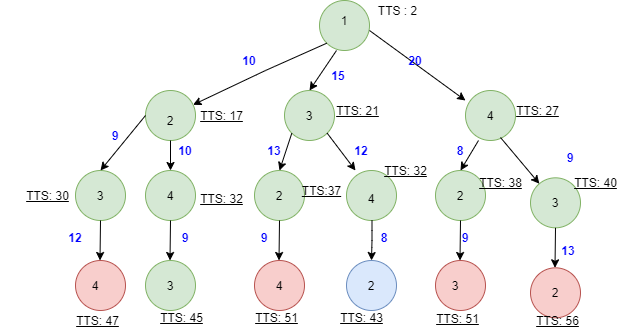
\includegraphics[scale = 0.7]{images/DynamicGraph.png}

\textbf{Result: Node 2.} \newline
Note that the best solution is the deepest node in the Graph with minimum TTS $<$ 46. 

\begin{itemize}
    
    \item \textbf{vPOI} is the \textbf{vector of pointers} containing the points of interest represented by the POI structure defined previously.
    \item \textbf{maxTime} is a variable containing the maximum time that a person can spend.
    \item \textbf{origin} parameter represents the position of the initial point at vPOI. 
    \item Always consider the \textbf{vPOI[0]} as the origin POI. 
\end{itemize}


    \begin{algorithm}[h]
    \caption{Traveling salesperson pre preprocessing}
    \begin{algorithmic}[1]
    
    \Procedure{preProcessing}{vPOI, maxTime, G=(V, E)}
    
        \For{i \textbf{from} 0 \text{to} $|$vPOI$|-1$}
            \State $vPOI[i] \gets \text{set visited false}$
        \EndFor
        \State $ $
        \State $minDistance \gets 0$
        \State $level \gets 0$
        \State $initialTime \gets time - \text{find time spend in vPOI[0]}$
        \State $ $
        \State $ $
        \Return $travelingSalesperson\text{(0, vPOI, $|$vPOI$|$, minDistance, initialTime, level)}$
    \EndProcedure
    \end{algorithmic}
\end{algorithm}
    \begin{itemize}
    \item \textbf{actualPoint} is the index of the actual point in \textbf{vPOI}
    \item \textbf{vPOI} is the \textbf{vector of pointers} containing the points of interest represented by the POI structure defined previously.
    \item \textbf{available} how many not visited points of interest in vPOI
    \item \textbf{minDistance} The minDistance until now. 
    \item \textbf{maxTime} The amount of time in minutes that a person still can spend
    \item \textbf{nodes} Quantity of nodes visited until now  
\end{itemize}
    
    \begin{algorithm}[H]
    \caption{Traveling salesperson dynamic approach}
    \begin{algorithmic}[1]
    
    \Procedure{travelingSalesperson}{actualPoint, vPOI, minDistance, maxTime, level, G=(V, E)}
        \State $maxLevel \gets{level}$
        \State $path \gets \text{vector}$
        \State $vPOI[actualPoint]\gets \text{set visited true}$
        \State $minDistance \gets \text{find time spent in this poi}$
        \State $ $ 
        
        \If {time $<$ 0}
        \State $minDistance \gets \infty$
        \State $ $
        \Return $emptyVector$, level, minDistance \Comment {There is no time left to visit this POI} 
        \EndIf 
        \State $ $
        \State $nodes \gets nodes + 1$ 
        \If {available $=$ 1}
        \Return $emptyVector$, level, minDistance \Comment {There is no more POIs to visit} 
        \EndIf
        \State $ $
        \newpage
        \For{i \textbf{from} 0 \text{to} $|$vPOI$|-1$}
            \If {vPOI[i] not visited}
                \State $actualDistance \gets 0$
                \State $auxLevel \gets level$

                \Comment{Calculating the available time left to spend}
                \State $srcPointIndex \gets \text{index of vPOI[actualPoint] in V}$
                \State $destPointIndex \gets \text{index of vPOI[i] in V}$ 
                \State $timeActualPOI \gets \text{find time spent in vPOI[i]}$
                \State $timeLeft \gets maxTime - dist[srcPointIndex][destPointIndex] - timeActualPOI$
                \State $ $
                
                \State $tempVector,nodesReached,actualDistance \gets travelingSalesperson(i, vPOI,\newline actualDistance, timeLeft, auxLevel)$
                
                \State $ $
                \State $ $
                \Comment{Update the actual distance}
                \State $actualDistance \gets actualDistance + pred[srcPointIndex][destPointIndex] + timeActualPOI$
                
                \State $ $
             
                \If {(minDistance $>$ actualDistance $and$ auxLevel $>=$ maxLevel)\newline $or$ (auxLevel $>$ maxLevel $and$ actualDistance $\neq \infty$ )}
                    \State $path \gets tempVector$
                    \State $minDistance \gets actualDistance $
                    \State $maxLevel \gets auxLevel$
                    \State $nextPOI \gets i$
                \EndIf
            \EndIf 
            \State $ $
            \If {nextPOI $!=$ -1} 
                \State $srcPointIndex \gets \text{index of vPOI[actualPoint] int V}$
                \State $destPointIndex \gets \text{index of vPOI[nextPOI] in V}$
                \State $level \gets maxLevel$
                \State $ $
                \State $floydPath \gets getFloydPath(srcPointIndex, desPointIndex)$
                \State $floydPath \gets floydPath[0...|floydPath|-1] + path[0... |path|-1]$  \Comment{Join the two vectors}
                \State $ $
                \State $ $
                \Return $floydPath, level, minDistance$
            \EndIf
            \State $ $ 
            \State $ $
            \Return $emptyVector, level, minDistance$
        \EndFor
    \EndProcedure
    \end{algorithmic}
\end{algorithm}
    
\newpage
\subsection*{Algorithm Analysis}  
\subsubsection*{Floyd-Warshall}
The time complexity for Floyd-Warshall is $O(|V^3|)$ and its space complexity is $O(|V^2|)$ as discussed before.
\subsubsection*{Greedy Approach}
\begin{itemize}
\item The time complexity of the algorithm is:
    \begin{center}
    $O(|V^3|)$ + $O(|V|)$ * $O(|V * log(V)|)$
    \end{center}
giving the final complexity of $O(|V^3|)$
\item The space complexity of the algorithm is:
    \begin{center}
    $O(|V^2|)$ + $O(|V|)$ * $O(1)$
    \end{center}
giving the final complexity of $O(|V^2|)$
\item The empirical analysis provided the following minimum, maximum and average times in ms after running the algorithm with 4x4, 8x8 and 16x16 grids passing by all nodes:
\begin{center}
\begin{tabular}{|c|c|c|c|} 
    \hline
     & 4x4 & 8x8 & 16x16 \\ [0.5ex] 
    \hline
    Maximum & 180 & 342 & 1503 \\ 
    \hline
    Average & 83 & 164 & 605 \\
    \hline
    Minimum & 36 & 78 & 332 \\
    \hline
\end{tabular}
\end{center}
\begin{figure}[h!]
    \centering
    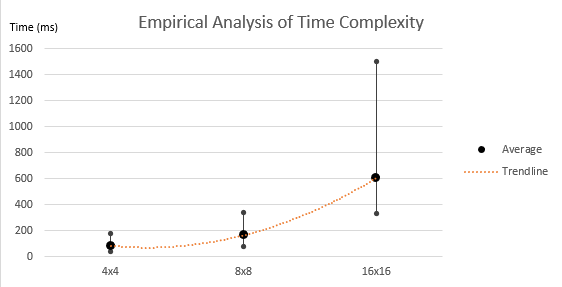
\includegraphics[width=0.6\linewidth]{graphic.png}
    \caption{A graphic done with the table information showing also the trendline.}
\end{figure}
\end{itemize}


\subsubsection*{Dynamic Approach}
\begin{itemize}
\item The time complexity of the algorithm is:
    \begin{center}
    $O(|V^3|)$ + $O(|V|)$ + $O(|V * V!|)$
    \end{center}
giving the final complexity of $O(|V * V!|)$
\item The space complexity of the algorithm is:
    \begin{center}
    $O(|V^2|)$ + $O(1)$ * $O(1)$
    \end{center}
giving the final complexity of $O(|V^2|)$
\end{itemize}

\newpage
\subsection*{Data Structures}
\subsubsection*{Nodes.csv}
The \textit{nodes.csv} file is a simple table of one column with all the nodes in the graph identified by it's id. 

\subsubsection*{Edges.csv}
\begin{itemize}
    \item $S_i$: Source, the id of the source node. 
    \item $T_i$: Target, the id of the target node. 
    \item $L_i$: Length of the road (in meters).
    \item $OSM id$: the id of the edge in the Open Street Map. 
    \item $Name$: name of the street in which the node belongs.
    \item $O_i$: Oneway, if the street is just one way.
    \item $M_i$: Maxspeed, the maxspeed of the road (in kilometres per hour).
\end{itemize}

\subsection*{POI\_cityName.txt}
Every city has a file called POI\_$<$cityName$>$.txt
\begin{itemize}
    \item $Name$: Name of each point of interest.
    \item $ID$: ID of the POI in the vector V of the Graph.
    \item $Time$: Time in minutes spent in the POI
\end{itemize}

\section*{Conclusion} 

The goal of this project was to develop a solution of the problem of route planning in a city sightseeing context. \par

For that purpose we resort to shortest-path and optimization algorithms as well as dynamic programming.\par

Finding a solution for choosing the next POI was hard and the greedy approach contains the fastest solution, however it's not the best one. By the other side, the dynamic approach finds the best solution, but it's very slow . \par

So, we decided that the best approach for our scenario would be: use the dynamic approach when the number of possible POI's is not much and the greedy approach when it's number is high. \par

The participation of each person is:
\begin{itemize}
\item Alexandre Abreu - 33\%

\begin{itemize}
    \item Algorithm
    \item Performance Tests
\end{itemize}

\item Eduardo Correia - 33\%

\begin{itemize}
    \item Input Data
    \item Graphical Interface
\end{itemize}

\item Juliane Marubayashi - 33\%

\begin{itemize}
    \item Input Data
    \item Algorithm
    \item Data Storage
\end{itemize}

\end{itemize}

\begin{thebibliography}{9}

\bibitem{OSMnx} 
Boeing, Geoff, \textit{OSMNnx}, Github repository, https://github.com/gboeing/osmnx

\bibitem{OpenStreetMaps} 
\textit{Open Street Maps}, https://www.openstreetmap.org/

\bibitem{Pandas}
\textit{Pandas}, https://github.com/pandas-dev/pandas

\bibitem{IntroductionToAlgorithms}
Cormen, Thomas H., and Thomas H. Cormen. 2001. \textit{Introduction to algorithms}. Cambridge, Mass: MIT Press.

\bibitem{FloydWarshal}
Sambol, Michael, \textit{Floyd-Warshal Algorithm in 4 minutes}, https://www.youtube.com/watch?v=4OQeCuLYj-4

\end{thebibliography}

\end{document}
https://www.overleaf.com/project/5e7e00fdae8f9200012cd123